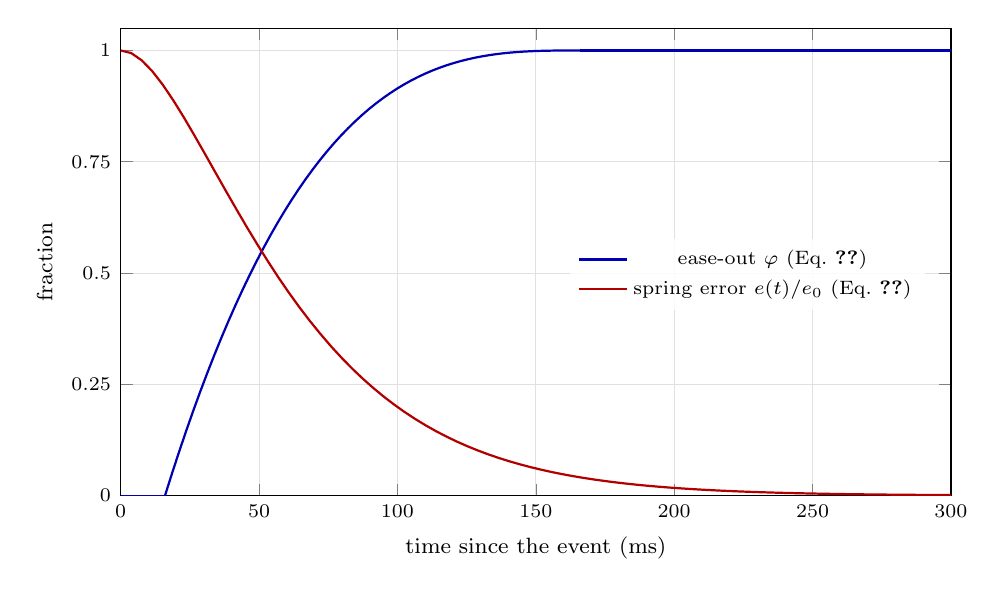
\begin{tikzpicture}
\begin{axis}[
  width=\columnwidth,height=0.62\columnwidth,
  xlabel={time since the event (ms)},ylabel={fraction},
  xmin=0,xmax=300,ymin=0,ymax=1.05,
  xtick={0,50,100,150,200,250,300},ytick={0,0.25,0.5,0.75,1},
  tick label style={font=\scriptsize},label style={font=\footnotesize},
  legend style={font=\scriptsize,at={(0.97,0.55)},anchor=north east,draw=none,fill=white,fill opacity=0.85,text opacity=1},
  grid=major,grid style={black!12},
  every axis plot/.append style={thick}
]
\addplot[blue!70!black,domain=16:166,samples=60] {1-(1-(x-16)/150)^3};
\addlegendentry{ease-out $\varphi$ (Eq.~\ref{eq:shown})}
\addplot[blue!70!black,forget plot] coordinates {(0,0) (16,0)};
\addplot[blue!70!black,forget plot,domain=166:300,samples=2] {1};
\addplot[red!70!black,domain=0:300,samples=80] {(1+0.03*x)*exp(-0.03*x)};
\addlegendentry{spring error $e(t)/e_0$ (Eq.~\ref{eq:spring})}
\end{axis}
\end{tikzpicture}
